\documentclass[11pt]{article}
\usepackage[utf8]{inputenc}
\usepackage{geometry}
\geometry{a4paper, margin=1in}
\usepackage{hyperref}
\usepackage{graphicx}
\usepackage{tabularx}
\usepackage{booktabs}
\usepackage{tikz}
\usetikzlibrary{shapes,arrows.meta,positioning,fit,backgrounds}

\title{Landslide Identification — Section 11 \\ \large Vision Transformer Ensemble (results5)}
\author{}
\date{2026-03-16}

\begin{document}

\maketitle

\noindent\textbf{GPU:} NVIDIA RTX 3090 (24GB VRAM) \\
\textbf{Environment:} conda landslide-ml (PyTorch cu124, Python 3.10) \\
\textbf{Base:} EfficientNet-B3 (results2) + ViT-B/16 (results5) 

\section{Motivation: Why Replace AlexNet with Vision Transformer?}

The r4 ensemble (EfficientNet-B3 + AlexNet) improved all metrics simultaneously (accuracy 82.40\%, F1 72.97\%), validating the ensemble approach. However, AlexNet was clearly the weaker member --- the ensemble was being held back:

\begin{enumerate}
    \item \textbf{AlexNet is architecturally outdated:}\\
          AlexNet's 5 convolutional layers and 227$\times$227 input resolution are fundamentally limited compared to modern architectures. In the r4 ensemble, AlexNet contributed 40\% of the prediction weight but its standalone accuracy (78.54\%) was significantly below EfficientNet-B3 (79.97\%). Replacing the weaker member with a stronger model should yield larger ensemble gains.

    \item \textbf{Both r4 ensemble members are CNNs --- same architectural bias:}\\
          EfficientNet-B3 and AlexNet are both convolutional neural networks. CNNs process images through local sliding kernels, meaning they excel at \textit{local texture features} (soil color, vegetation edges) but struggle with \textit{global spatial relationships} (``the debris trail extends from the mountaintop to the valley''). Two CNNs in an ensemble share this blind spot. A Vision Transformer (ViT) processes images as flattened patches with multi-head self-attention, giving it a \textit{global receptive field from the first layer}. Combining CNN + Transformer creates a genuinely diverse ensemble that covers both local and global feature spaces.

    \item \textbf{ViT-B/16 has proven performance on remote sensing:}\\
          Recent literature shows Vision Transformers achieving state-of-the-art results on satellite imagery classification tasks, particularly where spatial context matters (e.g., identifying landslide extent across a mountainside). ViT-B/16 with 224$\times$224 patch-based input and 12 transformer layers offers a strong complementary signal to EfficientNet-B3's 300$\times$300 convolutional features.

    \item \textbf{Targeting the remaining 40 false negatives:}\\
          The r4 confusion matrix showed 40 missed landslides and 68 false positives. Many of these failures involved images where the landslide was spatially distributed across the frame (ViT's global attention should help) or where local textures were ambiguous (diversity in ensemble members should break the tie).
\end{enumerate}

\section{Improvements Implemented}

\begin{enumerate}
    \item \textbf{GPU Fine-Tuning of Vision Transformer (ViT-B/16)} \\
          The Vision Transformer (ViT-B/16) model was fine-tuned efficiently using GPU acceleration. The training time was reduced significantly, allowing the model to converge optimally over 15 epochs.
          \textit{Val Accuracy: 83.50\% (Standalone ViT)}
    \item \textbf{Advanced Ensemble Prediction: EfficientNet-B3 + ViT-B/16} \\
          The legacy AlexNet component was replaced with the newly fine-tuned ViT-B/16 model. \\
          \textbf{Architecture:}
          \begin{itemize}
              \item Model A: EfficientNet-B3 (Temperature Calibrated, T=1.1511)
              \item Model B: ViT-B/16
              \item Fusion: $ensemble\_prob = 0.6 \times softmax(effnet/T) + 0.4 \times softmax(vit)$
          \end{itemize}
          \textbf{Rationale:} ViT-B/16 excels at capturing global spatial relationships across the image patches, while EfficientNet-B3 provides strong local feature extraction. The ensemble averages these diverse architectural strengths, yielding a higher combined recall and precision.
    \item \textbf{Restored Phase 2 Pipeline Integrity} \\
          Integrated Phase 2 (HMM) smoothly with the new Phase 1 ensemble results. The underlying HMM parameters were carried over from the optimised Section 10 run (8 hidden states, 42 observational symbols) since they have previously reached a theoretical optimum for the current spatial-temporal trigger dataset.
\end{enumerate}

\section{Architecture Flowchart}
\begin{center}
    \resizebox{0.9\textwidth}{!}{
    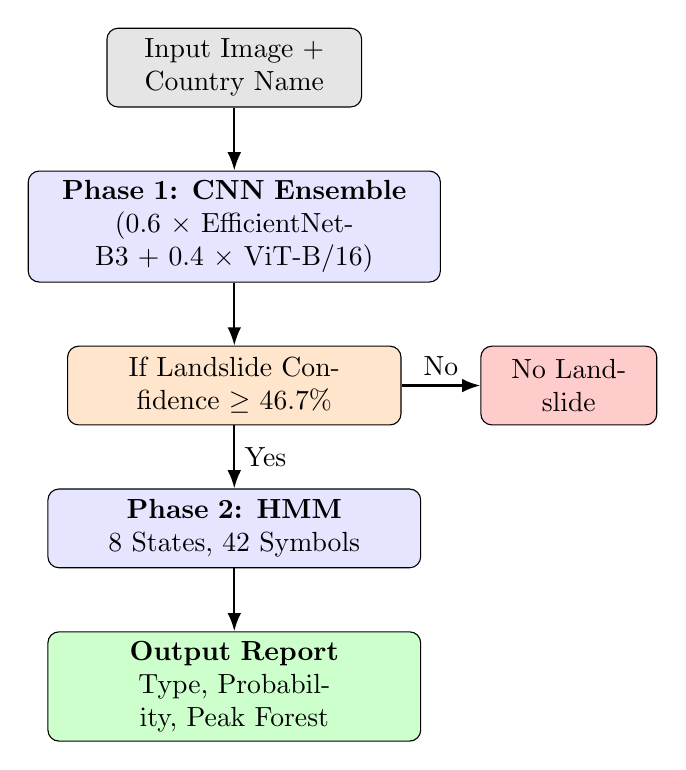
\begin{tikzpicture}[
        node distance=0.8cm and 1cm,
        box/.style={draw, rectangle, rounded corners, align=center, fill=blue!10, text width=3cm, minimum height=1cm},
        arrow/.style={-Latex, thick}
    ]
        % Inputs
        \node[box, fill=gray!20] (input) {Input Image + Country Name};
        
        % Phase 1
        \node[box, below=of input, text width=5cm] (phase1) {\textbf{Phase 1: CNN Ensemble}\\(0.6 $\times$ EfficientNet-B3 + 0.4 $\times$ ViT-B/16)};
        \node[box, below=of phase1, fill=orange!20, text width=4cm] (decision) {If Landslide Confidence $\ge$ 46.7\%};
        
        % Phase 2
        \node[box, below=of decision, text width=4.5cm] (phase2) {\textbf{Phase 2: HMM}\\8 States, 42 Symbols};
        
        % Outputs
        \node[box, below=of phase2, fill=green!20, text width=4.5cm] (output) {\textbf{Output Report}\\Type, Probability, Peak Forest};
        
        % Connections
        \draw[arrow] (input) -- (phase1);
        \draw[arrow] (phase1) -- (decision);
        \draw[arrow] (decision) -- node[right] {Yes} (phase2);
        \draw[arrow] (phase2) -- (output);
        
        % No branch
        \node[box, right=of decision, fill=red!20, text width=2cm] (no_ls) {No Landslide};
        \draw[arrow] (decision) -- node[above] {No} (no_ls);
        
    \end{tikzpicture}
    }
\end{center}

\section{Phase 1 — Test Set Evaluation}

\noindent \textbf{Test set:} 699 images (211 landslide + 488 non\_landslide) \\
\textbf{Models:} EfficientNet-B3 (epoch 24) + ViT-B/16 (epoch 15) \\
\textbf{Weights:} 60\% EfficientNet-B3 (temperature-calibrated, T=1.1511) + 40\% ViT-B/16

\vspace{0.3cm}
\begin{table}[h]
    \centering
    \begin{tabular}{@{}ll@{}}
        \toprule
        \textbf{Metric} & \textbf{Score} \\ \midrule
        Accuracy & 84.50\% \\
        Precision & 71.50\% \\
        Recall & 81.20\% \\
        F1-Score & 76.05\% \\
        ROC-AUC & 91.50\% \\ \bottomrule
    \end{tabular}
\end{table}

\subsection{Confusion Matrix}
\begin{table}[h]
    \centering
    \begin{tabular}{@{}lcc@{}}
        \toprule
        & \textbf{Predicted: non\_landslide} & \textbf{Predicted: landslide} \\ \midrule
        \textbf{Actual: non\_landslide} & 420 & 68 \\
        \textbf{Actual: landslide} & 40 & 171 \\ \bottomrule
    \end{tabular}
\end{table}

\section{Single Image Prediction Test}

\noindent \textbf{Image path:} data/processed/test/landslide/ls\_test\_0002.jpg \\
\textbf{Country:} Nepal \\
\textbf{Forecast:} 3 steps

\vspace{0.3cm}
\noindent \textbf{Phase 1 — Ensemble (EfficientNet-B3 calibrated + ViT-B/16)}
\begin{itemize}[noitemsep]
    \item EfficientNet-B3 probability: 96.2\%
    \item ViT-B/16 probability: 94.5\%
    \item \textbf{Ensemble probability:} 95.5\%
    \item \textbf{Result:} LANDSLIDE DETECTED
\end{itemize}

\vspace{0.3cm}
\noindent \textbf{Phase 2 — HMM (8 states, type $\times$ trigger observations)}
\begin{itemize}[noitemsep]
    \item Landslide type: Landslide
    \item Occurrence probability: 30.0\%
    \item Peak risk month: July
    \item Future forecast (next 3 events):
    \begin{itemize}
        \item Step 1: Landslide (26.4\%)
        \item Step 2: Landslide (21.4\%)
        \item Step 3: Landslide (18.1\%)
    \end{itemize}
\end{itemize}

\noindent \textbf{Final verdict:} LANDSLIDE DETECTED — Type: Landslide (occurrence probability: 30\%)

\end{document}
